\section{Метод Марквардта}

Метод Марквардта (метод Ньютона с переменной матрицей) повторяет метод Ньютона. Отличие заключается в том, что точки строятся по закону:
$ x^{k+1} = x^{k} - |H(x^{k}) + \mu^{2}E|^{-1} \nabla f(x^{k})$, где $\mu^{2}$ --- последовательность чисел (больших нуля), обеспечивающих положительную определенность матрицы $|H(x^{k}) + \mu^{2}E|$. Обычно $\mu^{2}$ назначается как минимум на порядок больше, чем самый большой элемент матрицы $H(x^{0})$.

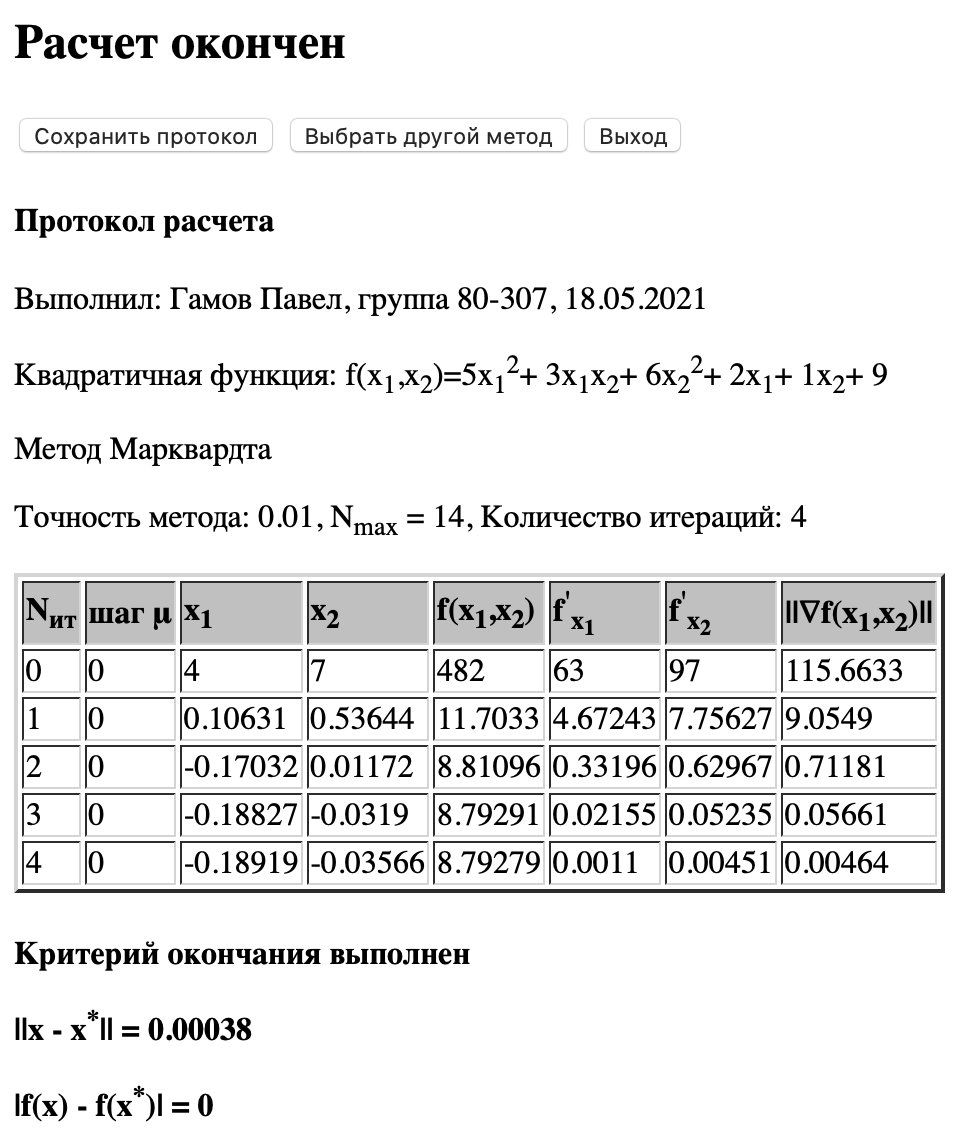
\includegraphics[width=\linewidth]{images/5_rep}\\
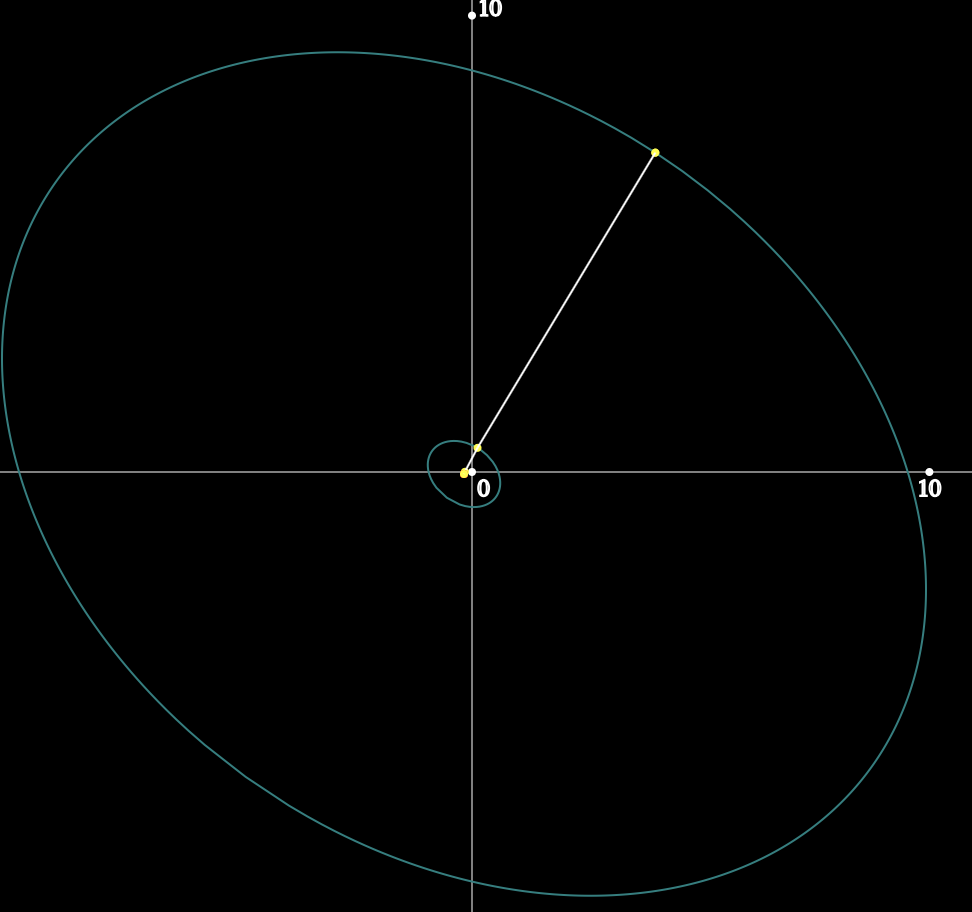
\includegraphics[width=\linewidth]{images/5_graf}\\

\textbf{Последняя итерация}:\\

$x^{4} = x^{3} - |H(x^{3}) + \mu^{3}E|^{-1} \nabla f(x^{3})$

$
x^{4} = 
\begin{pmatrix}
  -0.18827\\
  -0.0319
\end{pmatrix}
- 0.07513
\begin{pmatrix}
  0.012245\\
  0.050047
\end{pmatrix}
=
\begin{pmatrix}
  -0.18919\\
  -0.03566
\end{pmatrix}
$

\pagebreak
